%%==========================
%% Appendix 3: Jump Relation
%%==========================

\documentclass[../dissertation.tex]{subfiles}

\begin{document}

In this appendix we present an alternate proof of the jump relation 
\eqref{eq4:GFjump} which does  not utlize the formulas \eqref{eq1:GFrep}.

We begin by considering the integral 
\[
	\int_{\gamma} \frac{e^{i x \xi }}{\xi - \zeta(\lambda; \delta)\(1-e^{-2 \delta \xi} \)} \, \mathrm{d}\xi
\]
taken over the counterclockwise contour $\gamma$ shown below
\begin{center}
	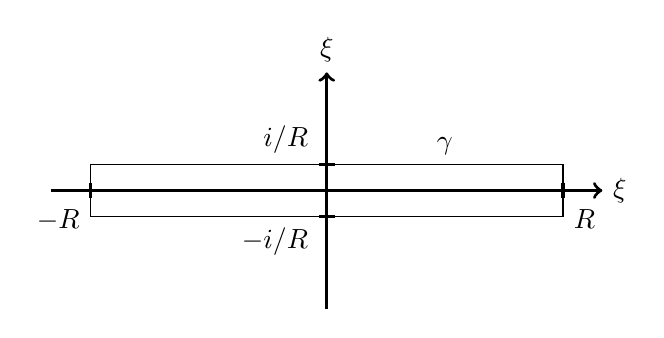
\begin{tikzpicture}[]
		\def\R{3}
		\def\xMax{3.5}
		\def\yMax{1.5}
		\def\tickLength{0.1}
		%% Axes
		\draw[->, very thick] (-\xMax, 0) -- (\xMax, 0) node[right] {$\re \xi$};
		\draw[->, very thick] (0, -\yMax) -- (0, \yMax) node[above] {$\im \xi$};

		%% Draw Contour
		\path (-\R, {1/\R}) edge (0, {1/\R})
			(0, {1/\R}) edge node[above] {$\gamma$}(\R, {1/\R})
			(\R, {1/\R}) edge (\R, {-1/\R})
			(\R, {-1/\R}) edge (-\R, {-1/\R})
			(-\R, {-1/\R}) edge (-\R, {1/\R});

		%% Draw Re axis tick marks
		\draw[very thick] (-\R, \tickLength) -- (-\R, -\tickLength) 
			node[below left] {$-R$};
		\draw[very thick] (\R, \tickLength) -- (\R, -\tickLength) 
			node[below right] {$R$};

		%% Draw Im axis tick marks
		\draw[very thick] (\tickLength, {-1/\R}) -- (-\tickLength, {-1/\R}) 
			node[below left] {$-i/R$};
		\draw[very thick] (\tickLength, {1/\R}) -- (-\tickLength, {1/\R}) 
			node[above left] {$i/R$};
	\end{tikzpicture}
\end{center}	
where 
\[
	\zeta(\lambda; \delta) 
		= \frac{\lambda}{1-e^{-\lambda \delta}}
		= \lambda \frac{e^{\lambda \delta}}{e^{\lambda \delta} - e^{-\lambda \delta}}
		= \frac{1}{2} \lambda e^{\lambda \delta} \csch{\lambda \delta}.
\]

To simplify notation, define
\[
	f(\xi) := f(\xi, x; \lambda, \delta) 
		:=  \frac{e^{i x \xi }}{\xi - \zeta(\lambda)\(1-e^{-2 \delta \xi}\)}.
\]
Since
\[
	|f(\pm R + iy)|
		= \left| 
				\frac{e^{\pm i xR} e^{-xy}}
					{\pm R + iy + \zeta(\lambda) \, e^{\mp 2 \delta R} e^{-2iy\delta} 
						- \zeta(\lambda)} 
			\right|
		\leq \frac{e^{-xy}}{|R^2 + y^2 + \zeta(\lambda) \, e^{ \mp 2 \delta R} - \zeta(\lambda)|}
		\to 0,
\]
as $R \to \infty$, it follows that
\[
	\lim_{R\to \infty} \int_\gamma f(\xi) \, \mathrm{d}\xi
		= \lim_{R\to \infty} \int_{-R + i/R}^{R + i/R} f(\xi) \, \mathrm{d}\xi
			+ \lim_{R\to \infty} \int_{-R - i/R}^{R - i/R} f(\xi) \, \mathrm{d}\xi
		= 2\pi \big(G_+(x) - G_-(x)\big).
\]
Thus, since 
\[
	\Res_{\xi = 0} f 
		= -\frac{e^{2 \delta  \lambda}-1}{2 \delta \lambda e^{2 \delta \lambda}-e^{2 \delta \lambda}+1},
\]
and
\[
	\Res_{\xi = \lambda} f 
		= \frac{\(e^{2 \delta \lambda }-1\) e^{i \lambda x}}{e^{2 \delta  \lambda} -2 \delta \lambda -1},
\]
we see from Cauchy's Residue Theorem that
\begin{align} \label{eq:1.02-ILW.GL-GR}
	G_L^+(x) - G_R^+(x)
		&= \frac{i \(e^{2 \delta \lambda }-1\) 
				e^{i \lambda x}}{e^{2 \delta  \lambda} -2 \delta \lambda -1}
			-\frac{i e^{2 \delta  \lambda}-1}{2 \delta \lambda e^{2 \delta \lambda}-e^{2 \delta \lambda}+1} \\
		&= i \alpha(\lambda; \delta) + i \beta(\lambda;\delta) e^{i\lambda x}, \nonumber
\end{align}
where
\[
	\alpha(\lambda; \delta) 
		:= \frac{1 - e^{-2\delta \lambda}}
			{1 - e^{-2 \delta \lambda} - 2\delta \lambda},
	\qquad \text{and} \qquad
	\beta(\lambda; \delta) 
		:= \frac{1-e^{-2\delta \lambda}}{1-2\delta - e^{-2\delta \lambda}}.
\]
In the limit $\lambda \to 0$ (\textit{i.e.} the pole at $\xi = \lambda$ collapses to the 
pole at $\xi = 0$), we find
\[
	\lim_{\lambda \to 0} G_L^+(x) - G_R^+(x) = - \frac{x}{\delta} + i\frac{2}{3}.
\]

\end{document}